\documentclass[aspectratio=169]{beamer}

% Needed packages
\usepackage{hyperref}
\usepackage{listings}
\usepackage{tabularx}

% Use the Fontys theme
\usetheme[lang=en]{Fontys}

\usepackage[backend=bibtex]{biblatex}
\addbibresource{references.bib}


% Title page settings
\title{Neo4j}
\institute{FHTenL}
\author{M. Gorlas, N. Adamavicius}

% Start the document
\begin{document}

% Create title page
\begin{titleframe}
    \titlepage
\end{titleframe}

\begin{frame}
    \frametitle{Roadmap}
    \tableofcontents
\end{frame}

\section{Data model and schema}
% Example frame for itemize
\begin{frame}
    \frametitle{Data model}
    Neo4j is a \textbf{graph database}.

    There are two main types of graph databases:
    \begin{itemize}
        \item Property graph model
        \item RDF graph model
    \end{itemize}

\end{frame}

\begin{frame}
    \frametitle{Property graph model}
    In Neo4j information is organized as nodes, relationship and properties.
\end{frame}

\begin{frame}
    \frametitle{Property graph model}
    In Neo4j information is organized as nodes, relationship and properties.

    \begin{figure}
        \centering
        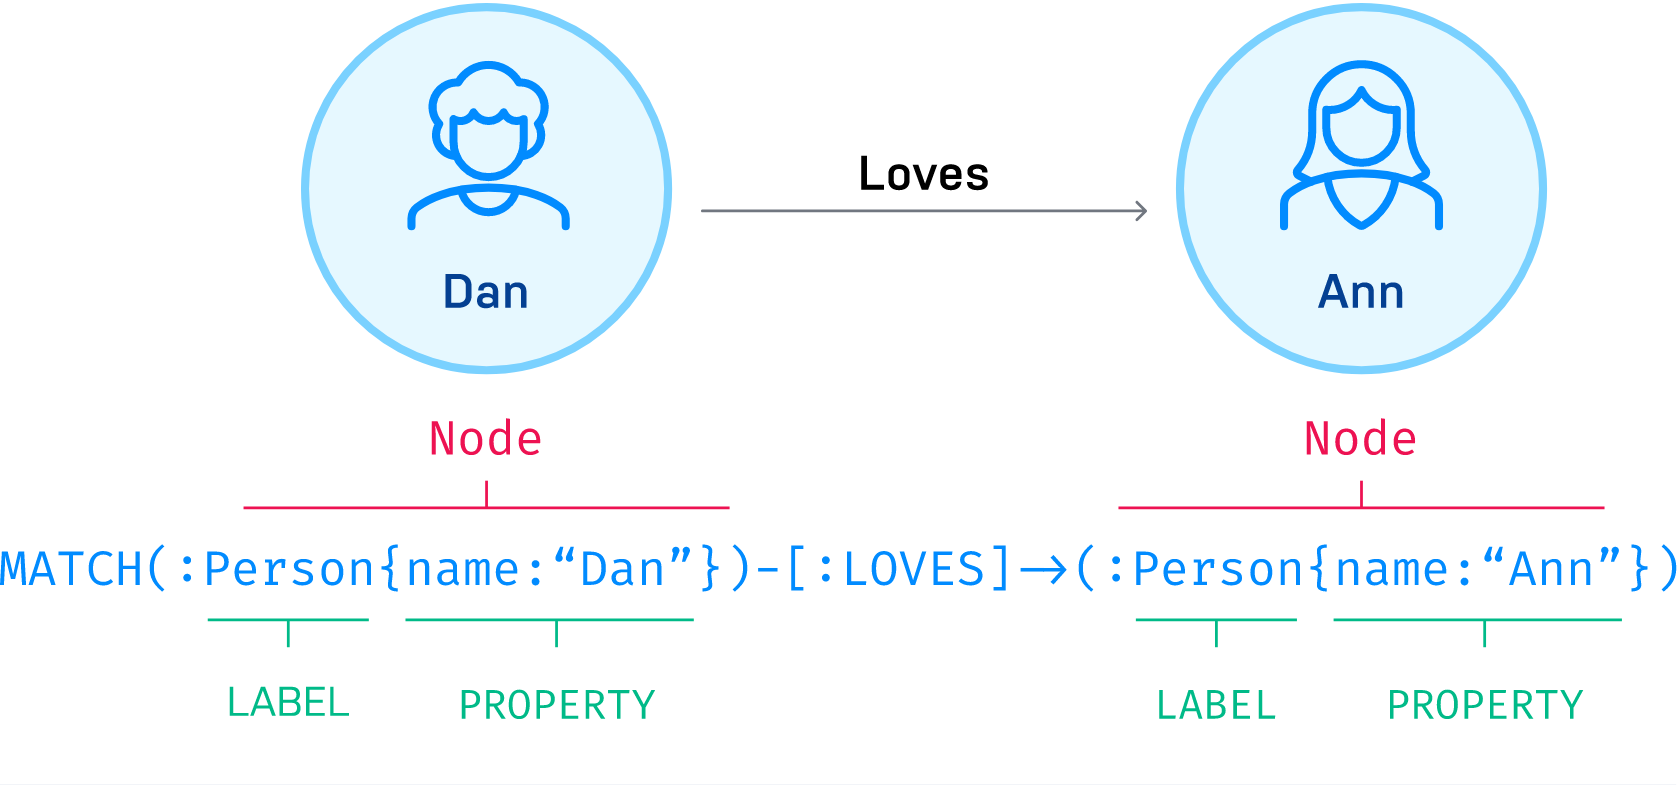
\includegraphics[width=0.4\textwidth]{pgmodel.png}
        \caption{Example of the property graph model \footfullcite{pgmodel}}
        \label{fig:pgmodel}
    \end{figure}

    In the property graph model, \textbf{nodes} are the \textbf{entities} in the graph.

    \textbf{Relationship} provide directed, named connections between two nodes entities.
\end{frame}

\begin{frame}[containsverbatim]
    \frametitle{Database schema}
    placeholder for now
\end{frame}

\section{Consistency and Replication}
% Example frame for URL
\begin{frame}
    \frametitle{Consistency}
	\begin{itemize}
   		\item Neo4j provides strong consistency.
		\item Neo4j employs causal consistency model.
		\item Isn't recommended DBMS when working with WAN.
	\end{itemize}
\end{frame}

\begin{frame}
	\frametitle{Replication}.
	\begin{itemize}
		\item Raft protocol.\footfullcite{raft-protocol}
		\item Leader/Follower Model.\footfullcite{leader-follower-model}
		\item High Availability.\footfullcite{high-availability}
	\end{itemize}
\end{frame}

\section{Security and Performance}

\begin{frame}
    \frametitle{Security}

    \begin{itemize}
        \item Schema-based Security \footfullcite{sbs}
        \item Role-based access control \footfullcite{ac}
    \end{itemize}
\end{frame}

\begin{frame}
    \frametitle{Schema-based Security}
    \begin{itemize}
        \item Protect the nodes and relationships by controling users' ability to traverse and read from different parts of the graph.
        \item Ensures that only authorized users have access to the data they need to protect sensitive data.
    \end{itemize}
\end{frame}

\begin{frame}
    \frametitle{Role-based access control}
    \begin{itemize}
        \item An approach, where you can apply restrictions to roles assigned to users at any level of granularity throughout the graph.
        \item Simplifies the task of assigning permissions and helps ensure that your data is secure.
    \end{itemize}
\end{frame}

\begin{frame}
    \frametitle{Performance}

    \begin{itemize}
        \item Compared to relational DBMS (MySQL in this case)
        \item Compared to other NoSQL DBMS
    \end{itemize}
    %Compare the performance of the DBMS with other DBMSs of the same and/or different
    %types (recent diagrams, give source, state how and what exactly was measured, be critical)
\end{frame}

\begin{frame}
    \frametitle{Compared to MySQL}

    Based on the benchmark using real-world data from Career Village, the experiment done by
    Rodrigues et. al, showed that Neo4j was faster than MySQL in most cases, particularly in
    pattern matching and recursive queries. However, MySQL has advantages in terms of data consistency
    and transactional support. 

    \begin{figure}
        \centering
        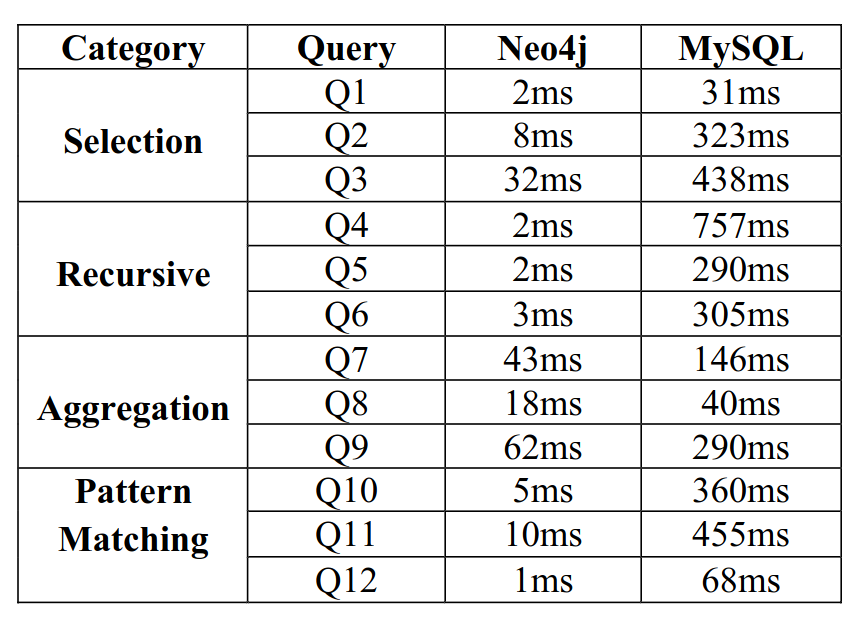
\includegraphics[width=0.3\textwidth]{bench1.png}
        \caption{Performance comparison between Neo4j and MySQL \footfullcite{mysql}}
        \label{fig:mysqlbench}
    \end{figure}
\end{frame}

\begin{frame}
    \frametitle{Compared to MySQL}
    In the benchmark the following types of queries were used:
    \begin{itemize}
        \item selection/search
        \item recursion
        \item aggregation
        \item pattern matching
    \end{itemize}
\end{frame}

\begin{frame}
    \frametitle{Compared to other NoSQL DBMS (1/2)}
    Based on the WDBench, a benchmark for graph databases focused on querying the Wikidata,
    Neo4j was the slowest of all tested graph databases, on all types of queries. \footfullcite{wdbench}

    \begin{figure}
        \begin{minipage}{0.48\textwidth}
            \centering
            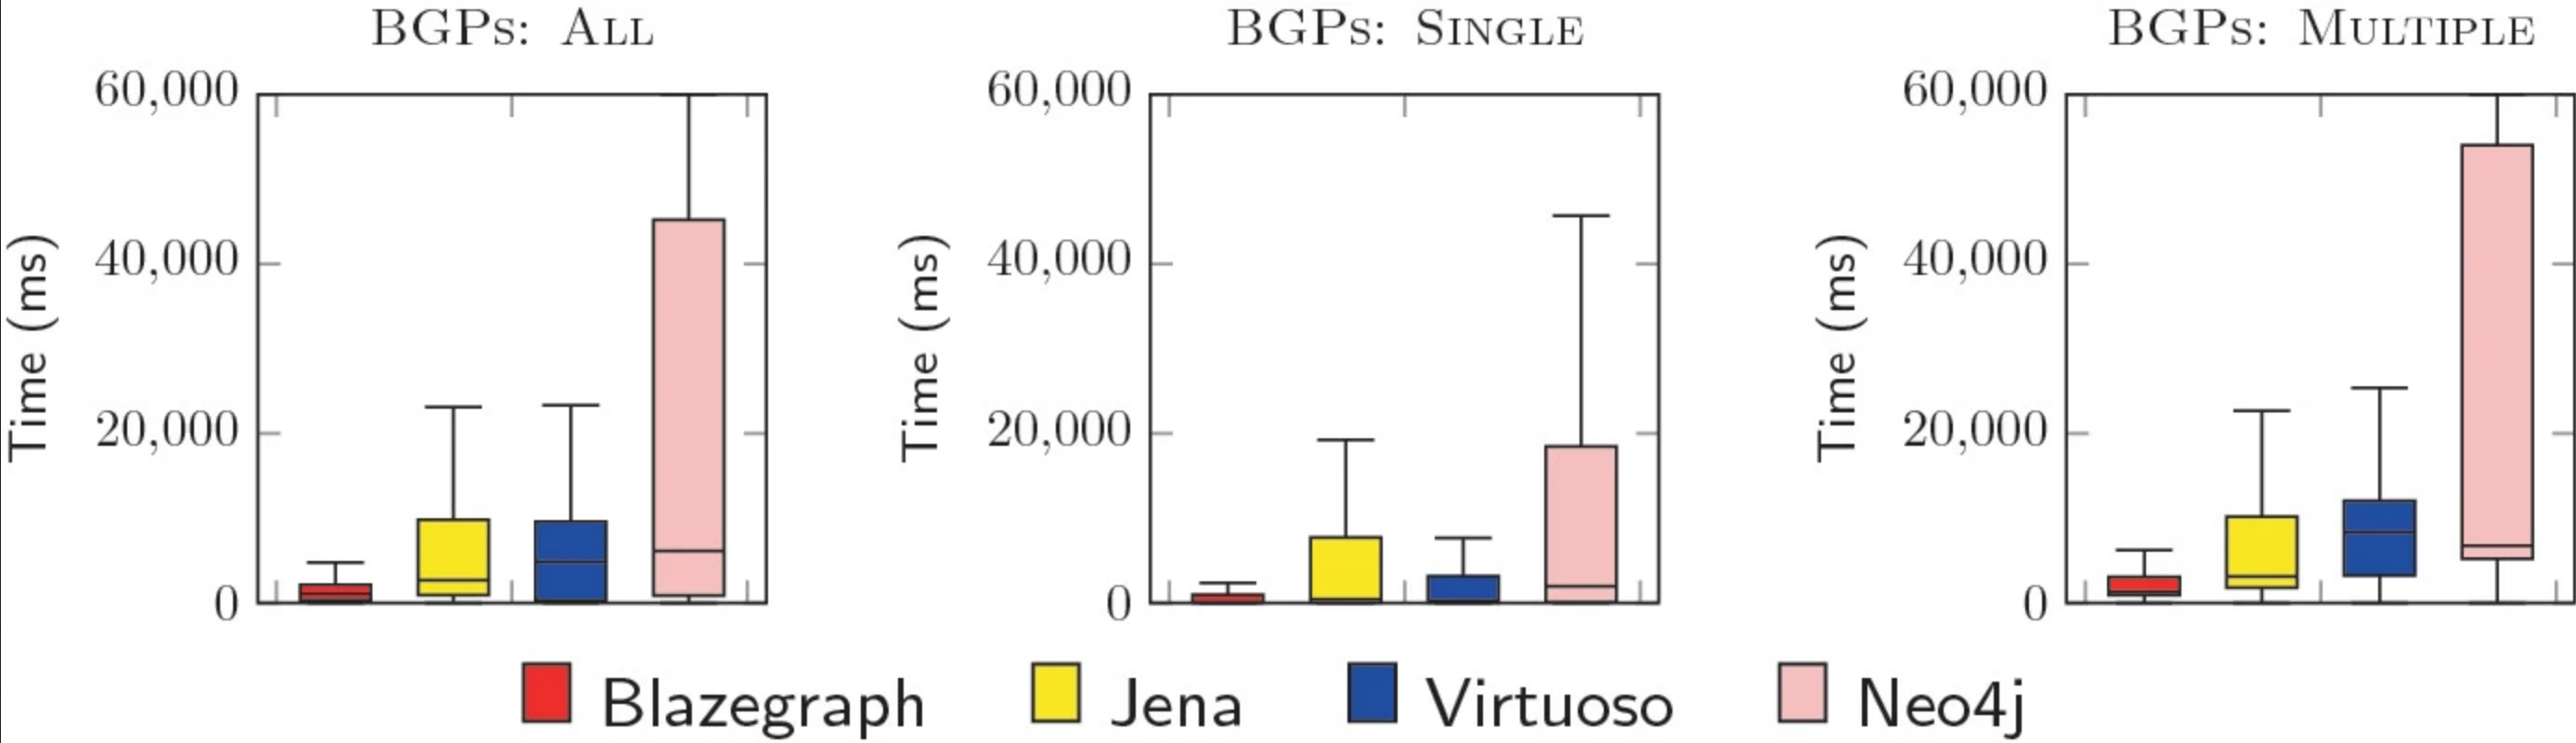
\includegraphics[width=\linewidth]{benchWD1.png}
            \caption{Basic Graph Patterns queries}
            \label{fig:bgp}
        \end{minipage}\hfill
        \begin{minipage}{0.48\textwidth}
            \centering
            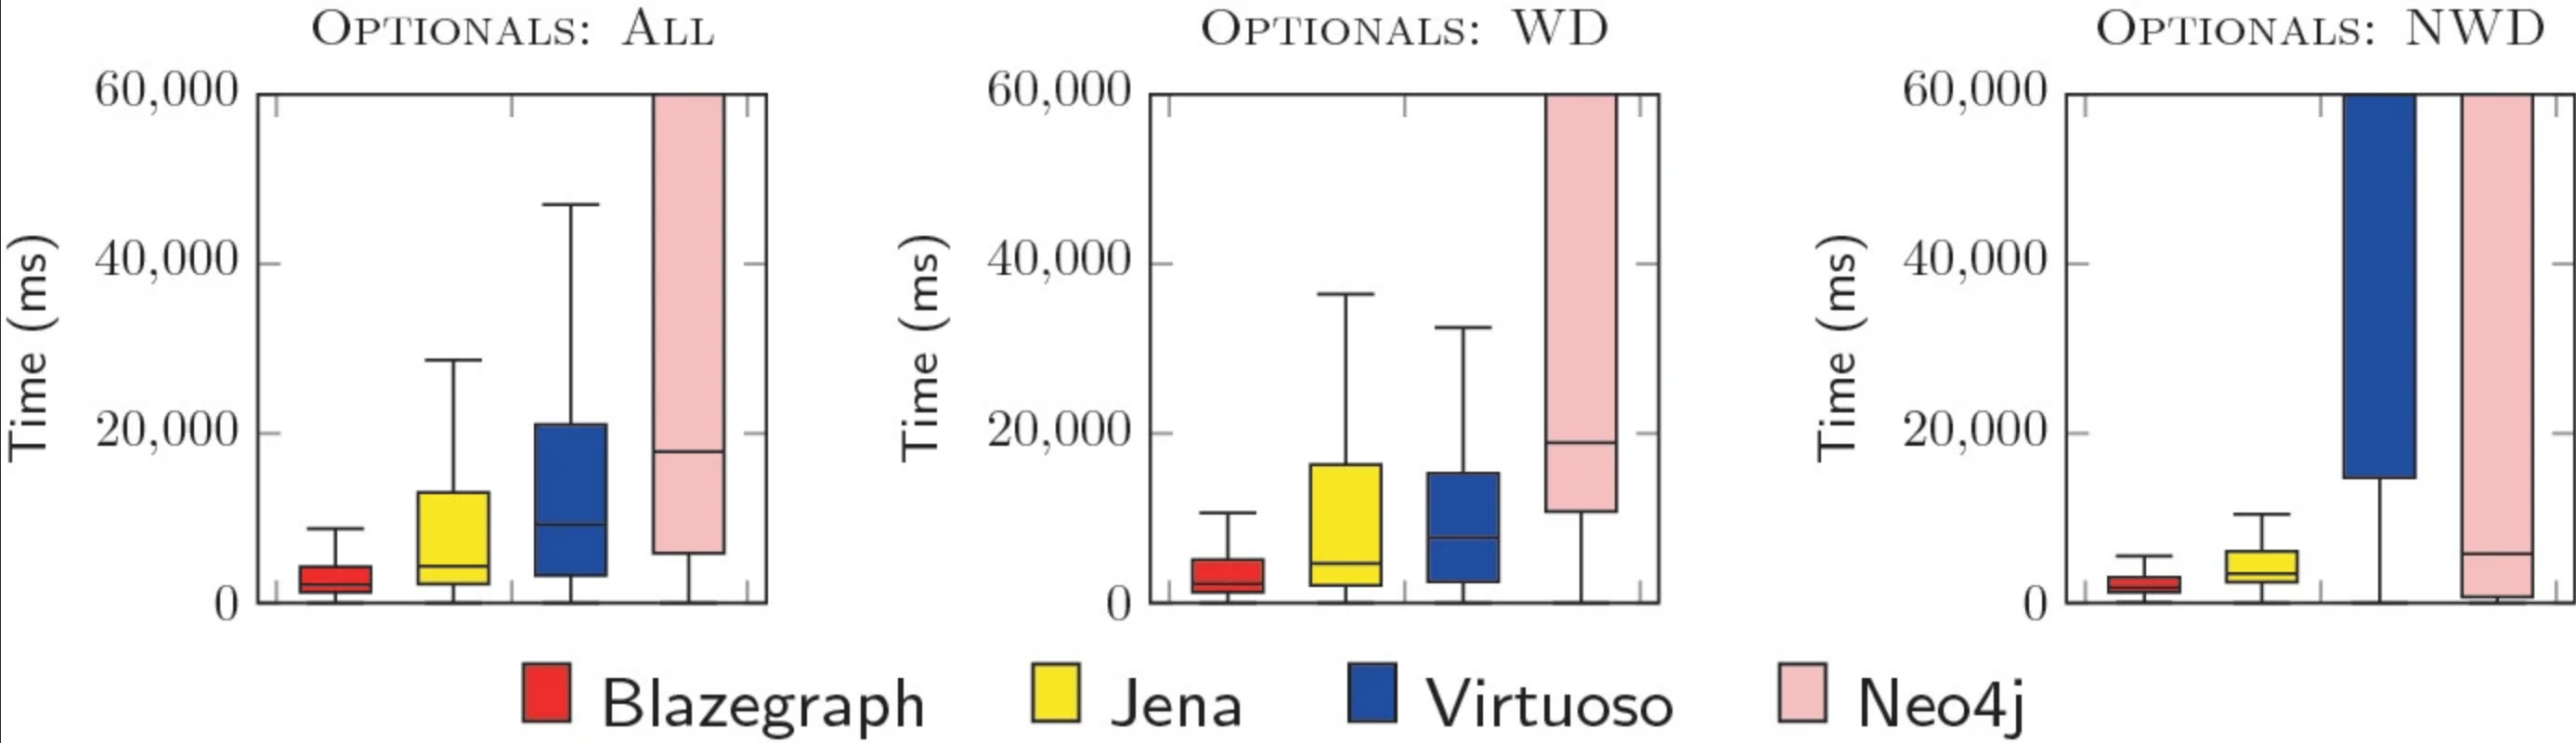
\includegraphics[width=\linewidth]{benchWD2.png}
            \caption{Optional Graph Patterns queries}
            \label{fig:ogp}
        \end{minipage}
    \end{figure}


\end{frame}

\begin{frame}
    \frametitle{Compared to other NoSQL DBMS (2/2)}

    \begin{figure}
        \begin{minipage}{0.48\textwidth}
            \centering
            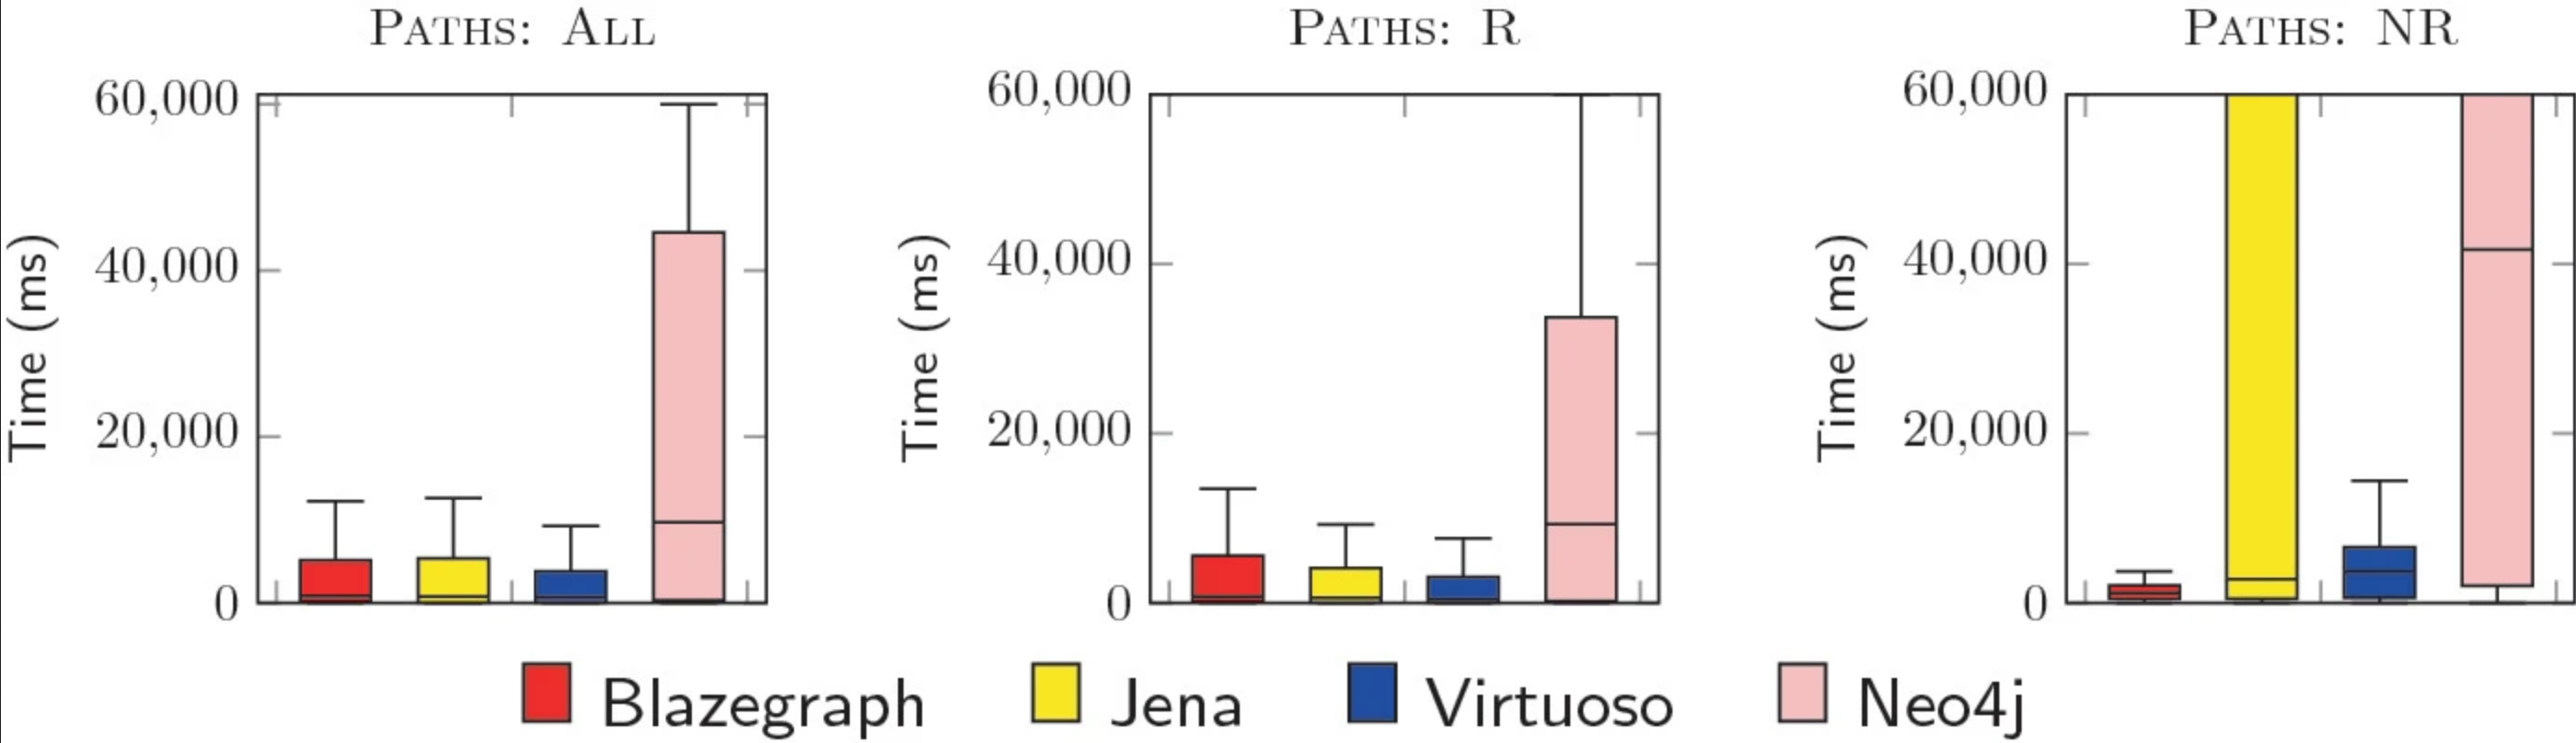
\includegraphics[width=\linewidth]{benchWD3.png}
            \caption{Path Patterns queries}
            \label{fig:path}
        \end{minipage}\hfill
        \begin{minipage}{0.48\textwidth}
            \centering
            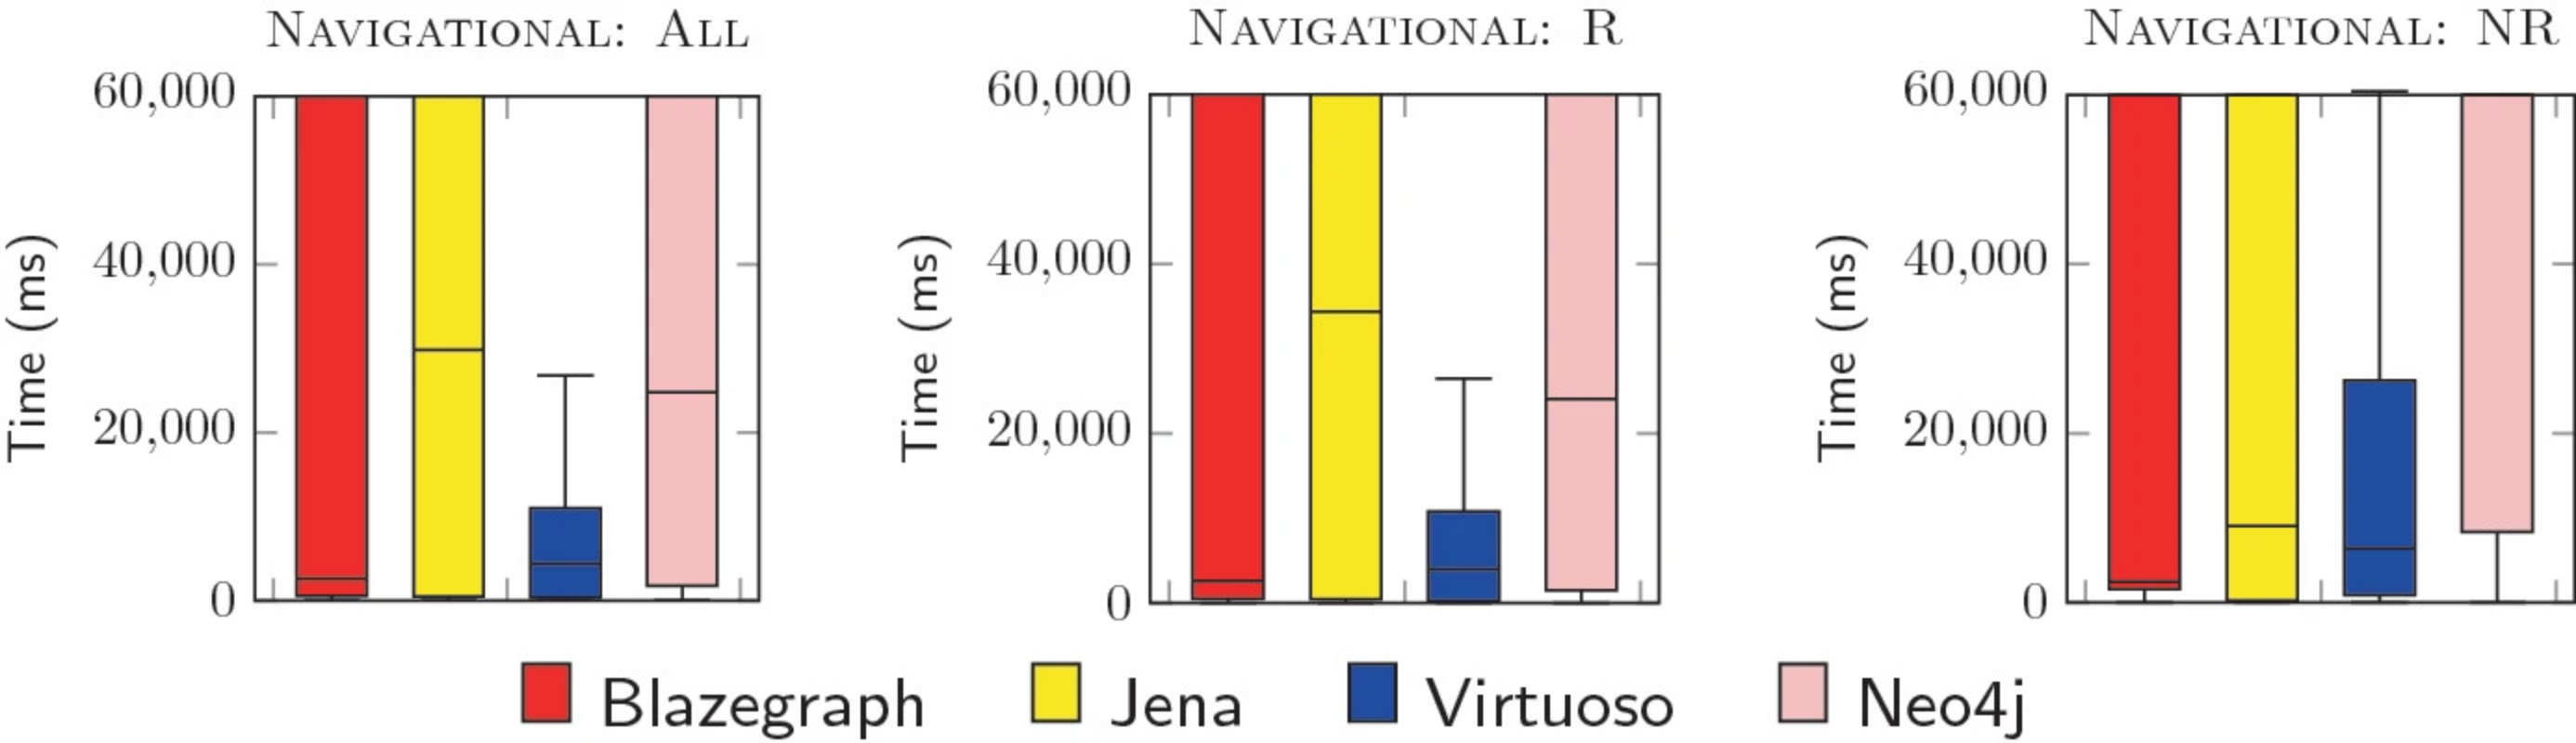
\includegraphics[width=\linewidth]{benchWD4.png}
            \caption{Navigational Graph Patterns queries}
            \label{fig:nav}
        \end{minipage}
    \end{figure}
    
\end{frame}


\section{Specific use cases and bit of history}

\begin{frame}
    \frametitle{Specific use cases}
	\begin{itemize}
		\item Knowledge Graphs.
		\item Recommendation Systems.
		\item Fraud Detection.
	\end{itemize}
\end{frame}

\begin{frame}
    \frametitle{Famous cases}
	\begin{itemize}
		\item NASA - uses the Neo4j knowledge graph to enhance its Lessons Learned Database, allowing engineers to identify trends and correlations between past projects and apply these insights to prevent future failures and improve decision-making.\footfullcite{nasa}
		\item eBay - utilizes Neo4j to power their chat bot recommendation system, enhancing user interactions with fast, context-aware responses and scalable graph database technology.\footfullcite{ebay}
		\item Fortune 500 Financial Services - uses Neo4j to visualize complex transaction relationships in real-time, enabling analysts to quickly detect and stop fraudulent activities, thereby saving thousands of dollars daily.\footfullcite{fortune500}
	\end{itemize}
\end{frame}

\section{Demo}

\begin{frame}
    \frametitle{Demo}
\end{frame}

\end{document}
